\documentclass[user_manual.tex]{subfiles}
\begin{document}
 \chapter{Primeros pasos}
 Antes de poner en funcionamiento a Justina, debemos conocer los software con los que trabaja y los requerimientos para  su correcto funcionamiento. También debes saber que Justina no funciona únicamente con una computadora, trabaja con 2 actualmente; una computadora esta integrada con ubuntu 14.04.1 (esta es la version ya probada), esta es la computadora principal, la cual se encargara de todos los procesos principales de Justina y tenemos la seguna computadora (plateada) integrada con windows 7, la cual únicamente se utiliza para la comunicación: el reconocimiento por voz y el habla de Justina\\
 \\
 Como primer paso se debe conocer el software básico para el funcionamiento de Justina.
 
 \section{Software básico}

Se requiere lo siguiente:\\
\\
-Ubuntu
\begin{itemize}
\item ROS Indigo desktop full
\item OpenNI + PrimeSense drivers
\item OpenCV 2.4.8 or 2.4.9. Compiled with OpenNi, WITHOUT OpenCL, WITHOUT Cuda, with Eigen
\item PCL 1.6
\end{itemize}

Para conocer la forma de instalar ROS, OpenNI, los drivers PrimeSense y OpenCV 2.4.9 por favor acude al apéndice B (software).\\
\\
-Windows 7
\begin{itemize}
\item Blackboard
\item SpRecV1
\item SpRecV2
\end{itemize}

La comunicacion entre las dos computadoras se da por medio de conexion ethernet, para esto se debe hacer una configuaración punto a punto. Para conocer la configuración de la red por favor visite el apendice de software.

 \section{Obtención del repositorio de Github}
 Como siguiente paso se debe obtener el repositorio de Justina con el que se ha trabajado Justina.\\
 \\
 Todos los paquetes del software de Justina se encuentran en Github.\\
Para descargar el repositorio lo que se debe hacer es lo siguiente: desde una terminal se debe clonar el repositorio  usado el siguiente comando:\\

\begin{minted}[
frame=lines,
framesep=1mm,
bgcolor=black,
baselinestretch=1.2
]{console}
 ~$ git clone https://github.com/RobotJustina/JUSTINA
\end{minted}
%$
 
\section{Instalación del software de Justina}
Una vez instalado ROS procedemos a instalar el software de Justina, para esto abrir una terminal y seguir las siguientes instrucciones:

\begin{enumerate}
 \item ingresamos a la carpeta JUSTINA y ejecutar JustinaSetup.sh
  \begin{center}
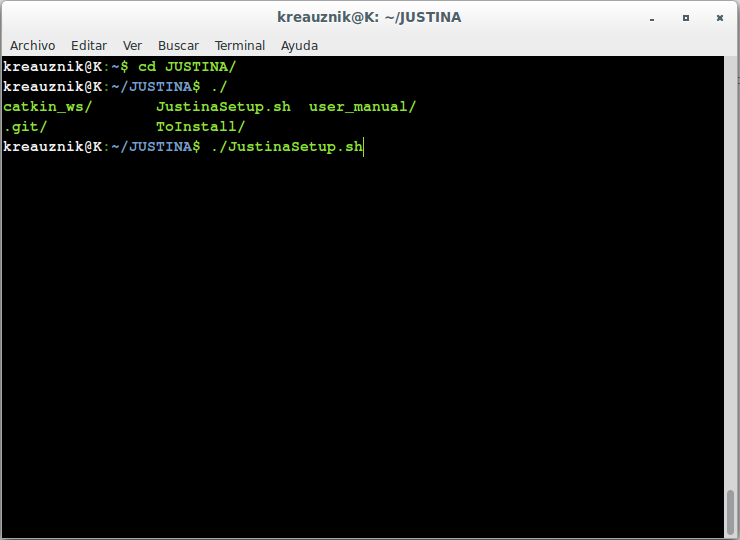
\includegraphics[width=0.73\textwidth]{Figures/PP/pp4.png}
\end{center}
 \item Aceptar cada que pregunte. Esto nos llevara varios minutos.
 \item Una vez instalado el software, debemos habilitar el uso de los puertos USB para ROS, para esto ingresamos al directorio "JUSTINA/ToInstall
 /USB (si quieres seguir las instrucciones más detalladamente, en la misma dirección abrir el archivo ``instructions'') una vez dentro
 de la carpeta ejecutar el siguiente comando:

\begin{minted}[
frame=lines,
framesep=1mm,
bgcolor=black,
baselinestretch=1.2
]{console}
 ~$ sudo cp 80-justinaRobot.rules /etc/udev/rules.d/
\end{minted}
%$ 
 
 \item Te pedirá la contraseña. Una vez termines de ejecutar el comando, se debe ejecutar el siguiente: 
 
\begin{minted}[
frame=lines,
framesep=1mm,
bgcolor=black,
baselinestretch=1.2
]{console}
 ~$ sudo udevadm control --reload-rules && sudo service udev restart
\end{minted}
%$
\begin{minted}[
frame=lines,
framesep=1mm,
bgcolor=black,
baselinestretch=1.2
]{console}
 ~$ && sudo udevadm trigger
\end{minted}
%$
 
\end{enumerate}
Listo, ya tienes instalado el software de Justina.

\section{Cómo compilar los repositorios de Justina}
Para compilar los paquetes de Justina simplemente ve al directorio " JUSTINA/catkin\_ws", en este directorio ejecutamos el siguiente comando: 

\begin{minted}[
frame=lines,
framesep=1mm,
bgcolor=black,
baselinestretch=1.2
]{console}
 ~$ catkin_make
\end{minted}
%$

Una vez compilados todos los paquetes, ejecutar el siguiente comando dentro del mismo directorio:

\begin{minted}[
frame=lines,
framesep=1mm,
bgcolor=black,
baselinestretch=1.2
]{console}
 ~$ source devel/setup.bash
\end{minted}
%$

 \begin{center}
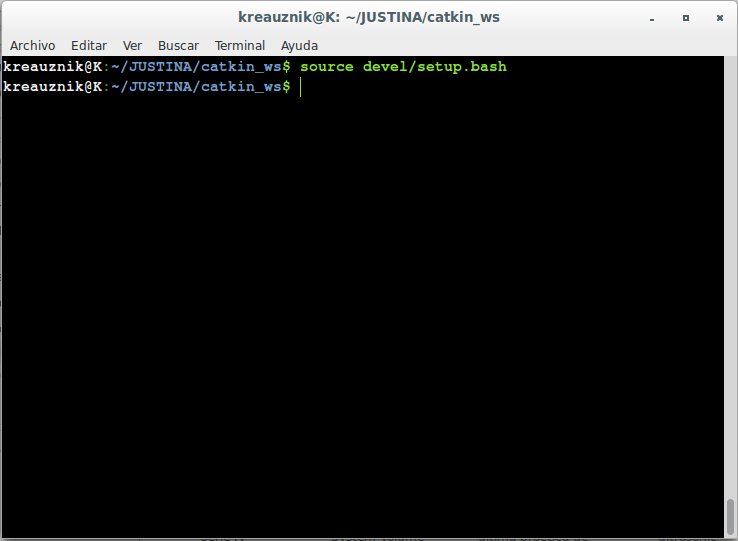
\includegraphics[width=0.73\textwidth]{Figures/PP/pp5.png}
\end{center}

Listo, ahora el software de Justina está instalado y los paquetes compilados y listos para usarse.

\section{RViz y GUI de Justina}
Para probar el funcionamiento del hardware y software de Justina utilizaremos RViz y la GUI. Para ejecutar estos programas utilizamos el 
comando:

\begin{minted}[
frame=lines,
framesep=1mm,
bgcolor=black,
baselinestretch=1.2
]{console}
 ~$ roslaunch surge_et_ambula justina.launch
\end{minted}
%$

 \begin{center}
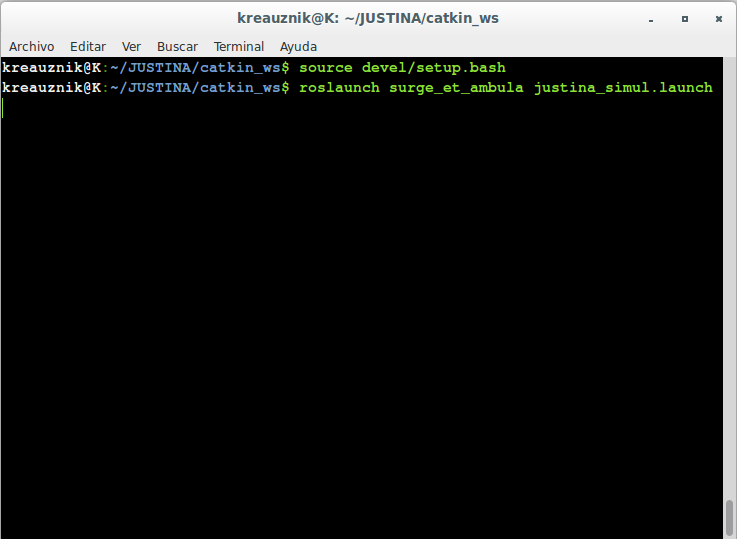
\includegraphics[width=0.73\textwidth]{Figures/PP/pp6.png}
\end{center}
\section{Simulación en el RViz y GUI de Justina}
Cuando no tenemos conectado el robot Justina a nuestras laptops lo único que podemos hacer
es simular a Justina en nuestras laptops, para esto ejecutamos el siguiente comando:
\begin{minted}[
frame=lines,
framesep=1mm,
bgcolor=black,
baselinestretch=1.2
]{console}
 ~$roslaunch surge\_et\_ambula justina\_simul.launch
\end{minted}
%$



\end{document}
